\documentclass{IEEEtaes}

\usepackage{color,array,amsthm}
\usepackage{graphicx}
\usepackage{dblfloatfix}   
\usepackage{amsmath}
\usepackage{algorithm}
\usepackage{algpseudocode}
\renewcommand{\algorithmicrequire}{\textbf{Input:}}
\renewcommand{\algorithmicensure}{\textbf{Output:}}
\newcommand{\algrule}[1][.1pt]{\par\vskip.2\baselineskip\hrule height #1\par\vskip.5\baselineskip}

\usepackage{soul}

\usepackage[outline]{contour}% http://ctan.org/pkg/contour
\usepackage[letterspace=50]{microtype}
\contourlength{0.2pt}
\contournumber{10}%

\jvol{03}
\jnum{2307668}
\jmonth{Fall}
\paper{1234567}
\pubyear{2023-24}
\doiinfo{}

\newtheorem{theorem}{Theorem}
\newtheorem{lemma}{Lemma}
\setcounter{page}{1}
%% \setcounter{secnumdepth}{0}

\begin{document}

\title{{\fontsize{22}{10}\selectfont \textbf{Variable Geometry}} \\ 
       {\fontsize{33.4}{10} \textbf{Truss Robot}} \\
       {\fontsize{24.9}{10} \textbf{Motion Planning} }\\
       on Irregular Terrain}


\author{OZGUR GULSUNA}
\member{}
\affil{Middle East Technical University, Ankara, TR} 

%% \author{FOURTH D. AUTHOR}
%% \affil{University of Colorado, Colorado, USA}

%% \receiveddate{}
%% \accepteddate{XXXXX XX XXXX}
%% \publisheddate{XXXXX XX XXXX}

\editor{}
\supplementary{}

\markboth{GULSUNA}{PRM PLANNING}



\maketitle

\begin{abstract}\st{\textls{This} paper explores the application of the Probabilistic Roadmap (PRM) algorithm in robot motion planning, focusing on a planar two-link robot navigating within a polygonal environment. The implementation details, including sampling methods, distance metrics, and collision checks, are discussed. Experiments involve varying link sizes, robot topologies, and obstacle configurations to adress the algorithm's adaptability and performance. Additionally, a specialized scenario is presented where a TARS-inspired robot navigates on a vertical plane, adhering to constraints simulating gravity effects. The results provide insights into PRM's effectiveness, optimality, and flexibility in handling diverse robot configurations and constrained environments.}
\end{abstract}

\begin{IEEEkeywords}\st{Motion Planning, Probabilistic Methods, Sampling Based Planning, 2D Environment, Matlab.}
\end{IEEEkeywords}
\vfill\null


\section{\normalsize INTRODUCTION}

{\scshape T}he Variable Geometry Truss (VGT) systems, characterized by linearly actuated truss members and passive rotational joints, faciliatate adaptability in various applications. Miura et al. introduced the foundational concept of VGT systems, primarily emphasizing fixed configurations \cite{miura}. Subsequent exploration of VGT as a modular and mobile system was undertaken by Hamlin et al. \cite{hamlin}, while Usevitch et al. contributed to the literature by introducing the kinematic analysis and optimization based locomotion of VGT systems \cite{usevitch}.



Our research builds upon this historical trajectory, culminating in the development of the Variable Topology Truss (VTT) system. Positioned as an evolutionary iteration of VGT, the VTT system represents an advancement that surpasses its predecessor's capabilities by enabling dynamic changes to the truss topology. This innovation is particularly instrumental in the context of search and rescue operations within disaster sites, where adaptability and versatility are paramount. VTT serves as an improved version of VGT, demonstrating the capacity to dynamically alter the configuration of the truss to optimize its functionality in complex and dynamic environments.

Fig. 1 provides a tangible representation of our scholarly pursuits—a hardware prototype and conceptual demonstration of the VTT system. The octahedral configuration chosen for locomotion studies aligns with the symmetry and impact-free rolling attributes, emblematic of its suitability for kinematic analysis and algorithmic development. While rooted in the kinematics and constraints of an octahedral VTT, our algorithmic framework is conceived with adaptability in mind, demonstrating its potential applicability to a broad spectrum of truss robots characterized by arbitrary configurations and triangular faces.

In summary, our research endeavors stand at the intersection of historical developments in VGT systems and the contemporary evolution represented by the Variable Topology Truss system. Positioned as a transformative force in adaptable robotic technologies, our work contributes both theoretically and practically to the ongoing discourse in the field




tochastic methods in robot motion control have proven to be effective in the literature. The introduction of randomness becomes particularly useful when searching for a solution in a vast configuration space, especially when dealing with robots that pose challenges for kinematics solutions. The core concept behind probabilistic methods is to randomly sample points from the free configuration space. As the number of samples increases, creating a local plan to connect these sampled configurations leads to the development of a global plan for the overall task. This method is especially advantageous in higher-dimensional worlds or robot configurations where calculation times are prolonged.

When comparing probabilistic approaches to more straightforward methods, it becomes evident that stochastic methods exhibit greater generalizability. Notably, by harnessing probabilistic completeness, these approaches effectively overcome limitations, navigating the configuration space with efficiency without the need to explicitly construct the configuration space itself to plan further. The crucial factor lies in formulating a sampling strategy based on a selected probabilistic function, generating multiple sample robot configurations within the free workspace. Despite the space and memory requirements entailed, the achieved probabilistic completeness positions this method as a successful motion planner suitable for navigating unrestricted worlds and intricate robot configurations. 

The paper will delve into this approach, initiating with the implementation of a simple probabilistic roadmap (PRM) planner designed for a planar two-link robot navigating within a polygonal world. The implementation details, including the sampling method, distance metric, and collision check aspects, will be explicitly addressed. The discussion will progress to the experimental settings, where the mentioned robot model is deliberately constrained, narrowing down the solution space. By focusing on the intricacies of the PRM planner's practical application to this specific robot scenario, the paper aims to provide a comprehensive understanding of the method's performance and adaptability in constrained environments.

\section{\large \textbf{Problem Definition}}

\begin{figure}[t!]
    \centering
    \vspace{0.5em}
\end{figure}

The initial step is to precisely construct the problem, which involves mathematically defining the robot, environment, and obstacles. When constructing these models, the structure is created so that the planar robot and the environment can be easily altered to facilitate widespread experiments. This adaptability aligns with the generalizability of the PRM method. This foundational step sets the stage for subsequent experiments, emphasizing the method's versatility in handling diverse robot configurations and environmental conditions.

% This work specifically engages with dimensions higher than two. This choice is deliberate, as navigating one-dimensional environments and obstacles presents a balance of being straightforward and complex simultaneously. Moreover, the notion of an "obstacle" itself poses a challenge to finding a "suitable path" solution in a single dimension. However, there exist a distinct research-area in the domain of list-type path planning tasks for deformable structures, as outlined in the literature \cite{one-dim}. Given these considerations, our primary focus is on higher dimensions, and dimensions lower than two are intentionally excluded from our current analysis.
% Implementation is carried on the simulation environment created in MATLAB. The 2D field has dimensions that are ten by ten units. There is a single start node and a single goal. The obstacle number is altered but finite and the workspace is bounded. The bug or in our case the probe is a point object with rotational range sensor that has a finite range. 

\subsection{{\fontsize{11}{10}\selectfont R}OBOT CONFIGURATION}

The robot have a multiple rigid links each connected to the previous one with a rotational joint and the joint location is selected from the previous link, as depicted in the Fig.~\ref{robot}.

\begin{figure}[h!]
    \begin{center}
        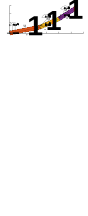
\includegraphics[width=0.85\linewidth]{figures/[1]ROBOT.pdf}
     \end{center}
     \caption{Robot configuration, $L_i$ and $W_i$ are link lengths and widths.}
     \label{robot}
\end{figure}

For the adjustment of individual lengths and widths, along with the addition of any number of links with individual joint locations. This flexibility facilitates the generation of a variety of robot topologies, as depicted in Fig.~\ref{topologies}. However, it's important to note that the constructed robots cannot form closed chains, as doing so requires solving kinematic equations to enable movement. This limitation becomes a topic for further discussion and exploration in future work.

The configuration space for the robots, that having multiple links, is in the form of $R^2*S^1*S^1*...*S^1$. This configuration can be represented with $q = [ x \ y \ \theta_1 \ \theta_2 \ ... \ \theta_n ]$. The angles in clockwise direction and allow for the full rotation without the robot colliding with itself, one can think about it as the links are on different planes.

% \begin{algorithm}[t]
% \caption{Rotational Plane Sweep Range Sensor}
% \label{alg:rps_sensor}
% \begin{algorithmic}
% \Require $robot\_position(v),$ $arena\_map$
% \Ensure $distance$, $angle$
% \algrule
% \If{robot is out of bounds}
%     \State exit.
% \EndIf
% \State $\mathcal{E} \gets$ number of vertices $\in \ \mathcal{Q}$
% \State $\mathcal{S} \gets$ ordered edges $\in \ \mathcal{Q}$
% \For{\text{$v:$ robot position}} 
%     \If{$v_i$ is visible to $v$}
%         \State Add the edge ($v$,$v_i$) to visibility graph
%     \EndIf
%     \If{$v_i$ is the beginning of an edge, $E$ $\notin$ $\mathcal{S}$}
%         \State insert $E$ into $ \mathcal{S}$
%         \State calculate dist, angle $E$ to $v$
%     \EndIf
%     \If{$v_i$ is the end of and edge in $\mathcal{S}$}
%         \State delete the edge from $\mathcal{S}$
%     \EndIf
% \EndFor

% \end{algorithmic}
% \end{algorithm}

\begin{figure}[b]
    \vspace{-2em}
    \begin{center}
        \includegraphics[width=0.85\linewidth]{figures/TOPOLOGIES.pdf}
     \end{center}
     \caption{Various robot structures with different number of links.}
     \label{topologies}
\end{figure}

\subsection{{\fontsize{11}{10}\selectfont W}ORKSPACE CONFIGURATION}

The workspace comprises a planar map bounded by an adjustable-size rectangle. Planar obstacles, taking the form of polygonal shapes, are placed to restrict the robot's freedom within this workspace. Both the initial and goal configurations are predefined, with careful consideration to ensure they avoid collisions with the obstacles initially. Notably, the obstacles are static and shapes remain constant over time without any variations. Unlike a grid-based structure, the workspace is not laid out over a grid, freeing the sampling process from dependence on such a structured grid for selection. This characteristic allows for a more flexible and adaptive sampling approach in navigating the robot through the dynamic environment.


\section{\large \textbf{Probabilistic Roadmap Planning}}
The fundamental PRM algorithm, extensively detailed in the reference book \cite{choset}, can be summarized as a multi-step process. Initially, the PRM method start by generating a set of robot configuration samples within the free workspace. After ensuring collision-free configurations, the algorithm proceeds to connect these samples, now referred to as nodes, to other nodes. During this connectivity phase, the PRM algorithm rigorously checks for collision-free transitions between nodes. Each such transition is identified as an edge, and the determination of the number of these edges involves considering the neighboring k nodes. In essence, the PRM method constructs a network of nodes and edges, effectively representing a roadmap that captures feasible paths through the configuration space while addressing collision constraints. The important aspect comes in when the algorithm does not need a precise description of the workspace obstacles. This approach provides a versatile and scalable solution for robot motion planning in complex environments.

% The subsequent sections will dvelve into the details about the implementation and how the algorithm is used with 

\subsection{\fontsize{10}{13}\selectfont LOCAL PLANNER}
The initial phase of the PRM approach involves sampling the workspace, a critical step in constructing a comprehensive roadmap for robot motion planning. For a more thorough exploration, a local planner is implemented. This local planner employs a systematic approach: it randomly samples throughout the entire workspace, and if a collision is encountered during this sampling process, the respective sample is discarded. The randomness in the sampling step is achieved by utilizing the random function, without any modifications or altering the sampling density.

The randomly generated samples in this context represent distinct configurations of the form $q = [ x \ y \ \theta_1 \ \theta_2 \ ... \ \theta_n ]$ . Each sample corresponds to a random configuration in the configuration space, and these samples are subsequently referred to as nodes for further reference. The sampling process continues until the required sample count is reached, with each generated configuration is valid and adheres to the defined constraints. 

The sample count serves as a critical parameter in PRM implementation, influencing the quality and efficiency of the obtained solutions. In general, a higher sample count tends to yield more optimal solutions. However, this comes at the cost of increased memory and computational intensity, impacting not only the sample generation phase but also subsequent steps in the algorithm. As the difficulty of the problem increases—signified by a generated sample count an order of magnitude higher than the useful or applicable samples for the solution—it becomes necessary to use a larger number of samples. This ensures a more comprehensive exploration of the configuration space, increasing the likelihood of encountering useful samples in complex scenarios. In the experimentation , varying sample numbers are explored to understand their impact on solution quality and computational efficiency.

\begin{figure}[t]
    % \vspace{-1.5em}
    \begin{center}
        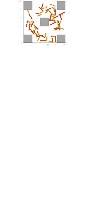
\includegraphics[width=0.9\linewidth]{figures/LOCALPLANNER.pdf}
     \end{center}
     \vspace{-1.5em}
     \caption{30 Samples generated with the local planner.}
     \label{samples}
     \vspace{-1em}
\end{figure}

\subsection{\fontsize{10}{13}\selectfont COLLISIONS AND LOCAL PATHS}
In the sampling step, collision checks are conducted straightforwardly by checking the intersection of generated configurations. This collision check is implemented using MATLAB's polyshape intersect function. The same function is employed for the inbounds check, creating a box with a hole on the outer perimeter of the map, ensuring that the generated samples remain within the valid workspace. This approach is both intuitive and efficient.

Once the samples are generated strictly within the free workspace, the next process involves establishing local connections which is more intricate.  It requires interpolating between configurations that are to be connected and checking for collisions at each interval. The process is depicted in the Fig~\ref{local-path}. While this approach may seem time-consuming, it ensures a thorough assessment of the trajectory's safety. This collision check ensures the feasibility of local connections.

Two techniques have been implemented to improve the computational efficiency of collision algorithms. The first technique checks whether two configurations are within each other's line of sight. This mechanism is employed just before the path interpolation. If the check results in a failure, the path interpolation is halted, and the path is discarded.

In second method, the collision check sequence is terminated whenever a collision is detected. The subsequent intervals are not checked. This strategy reduces unnecessary computational overhead, which is particularly necessary since this process being the most time consuming part of the PRM algorithm.

\begin{figure}[b]
    \vspace{0.75em}
    \begin{center}
        
\includegraphics[width=0.9\linewidth]{figures/LOCALPATH.pdf}
     \end{center}
     \caption{Local path collision check, between neighboring two nodes.}
     \label{local-path}
\end{figure}

\begin{figure}[t]
    % \vspace{-1.5em}
    \begin{center}
        \includegraphics[width=0.9\linewidth]{figures/ROADMAP.pdf}
     \end{center}
     \vspace{-1.5em}
     \caption{Generated roadmap for the 30 sample environment.}
     \label{roadmap}
    \vspace{-1em}
\end{figure}

\subsection{\fontsize{10}{13}\selectfont DISTANCE METRIC}
After establishing a method to disregard unusable paths, there exists another step precedes the construction of the roadmap. This step involves defining a metric that proves invaluable when comparing different paths, particularly in high-dimensional spaces. The robot configurations are represented as a combination of Euclidean distances in a plane, that are in $x-x'\ ,\ y-y'$ and angle differences corresponding to the number of links, $\theta_1-\theta_1' \ , \theta_2 - \theta_2' \ , \ ... \ , \theta_n - \theta_n'$. 

This configuration divide results in two distinct groups: translation and rotation. In constructing a distance metric, the introduction of different weights $W$ for each group is intended to guide the algorithm toward achieving the desired motion. With this approach, a "distance" between any two configurations can be calculated, however we will use it only for the nodes that are connectable.

% \begin{equation}
% \end{equation}

\subsection{\fontsize{10}{13}\selectfont CONSTRUCTING THE ROADMAP}
The groundwork and essential components have been established to pave the way for constructing the roadmap. This roadmap, functioning as a connection graph, is comprised of nodes or configurations situated in the free space. These nodes are interconnected through path collision checks, and the weights of these connections are determined by the distances between nodes. Essentially, the nodes represent configurations, and edges are formed between them if the connection does not result in a collision. It's noteworthy that the generated edges may be either unidirectional or bidirectional, contingent on collision checks for both forward and backward directions. This aspect is influenced by the periodicity of link rotation with respect to $2\pi$.

As the number of samples increases, the potential combinations for checking connections between nodes grows exponentially. To mitigate this problem, a method is employed to connect local nodes exclusively. Each node is examined for a fixed number, $K$, of neighboring edges. This constraint significantly reduces the number of potential combinations, resulting in a more manageable and computationally efficient solution. By focusing on local connections, the algorithm can prioritize relevant paths, offering a more generalizable and scalable approach.

\begin{figure*}[b!]
    \begin{center}
        \includegraphics[width=1\linewidth]{figures/EXP1-1.pdf}
     \end{center}
     \vspace{-1em}
     \caption{Single bar planning, left is the constructed roadmap, the right is the path for the solution.}
     \label{bar-1}
     \vspace{-1em}
\end{figure*}

\begin{figure*}[t]
    \begin{center}
        \includegraphics[width=1\linewidth]{figures/EXP1-2.pdf}
     \end{center}
     \vspace{-1em}
     \caption{Single bar planning, the goal configuration is rotated 180 degrees, solution is more straightforward.}
     \label{bar-2}
     \vspace{-1em}
\end{figure*}

\begin{figure*}[t]
    \begin{center}
        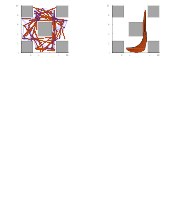
\includegraphics[width=1\linewidth]{figures/EXP1-3.pdf}
     \end{center}
     \vspace{-1em}
     \caption{Single bar planning, the sample space is constrained with the new obstacles.}
     \label{bar-3}
     \vspace{-1em}
\end{figure*}

\subsection{\fontsize{10}{13}\selectfont DIJKSTRA'S ALGORITHM}
The resultant weighted graph can be solved with various algorithms. The employed method utilizes Dijkstra's Algorithm, which is explained in more detail in~\cite{dijkstra}. This algorithm finds the sequence of nodes from any starting node to any destination node. In the implemented method, the first node is designated as the start node, and the last node is appended as the goal node. The pseudocode for the algorithm is provided below.

\vspace{-0.5em}

\begin{algorithm}
\caption{Dijkstra's Algorithm}
\begin{algorithmic}[1]
\Function{Dijkstra}{$G, \text{source}$}
    \ForAll{$v$ \textbf{in} $G.\text{Vertices}$}
        \State $\text{dist}[v] \gets \infty$
        \State $\text{prev}[v] \gets \text{undefined}$
        \State \textbf{add} $v$ \textbf{to} $Q$
    \EndFor
    \State $\text{dist}[\text{source}] \gets 0$
    
    \While{$Q$ is not empty}
        \State $u \gets$ vertex in $Q$ with min $\text{dist}[u]$
        \State \textbf{remove} $u$ \textbf{from} $Q$
        
        \ForAll{$v$ \textbf{in} neighbors of $u$ still in $Q$}
            \State $\text{alt} \gets \text{dist}[u] + G.\text{Edges}(u, v)$
            \If{$\text{alt} < \text{dist}[v]$}
                \State $\text{dist}[v] \gets \text{alt}$
                \State $\text{prev}[v] \gets u$
            \EndIf
        \EndFor
    \EndWhile
    
    \State \Return $\text{dist}[], \text{prev}[]$
\EndFunction
\end{algorithmic}
\end{algorithm}

\vspace{-2.2em}
\section{\large \textbf{Experiments}}
The experiments are designed to find a balance between time-complexity and solution feasibility. The initial two experiments explore different link sizes and variations in robot topologies. Each sub-experiment aim observe the impact of sample count and neighbor number on the planning process. However, in certain instances, distinguishing the specific causes behind observed differences in results can be challenging, as multiple factors may contribute concurrently.

\subsection{\fontsize{10}{13}\selectfont EXPERIMENT-1}
The first experiment involves a single long bar that can move and rotate within a plane, and the objective is to guide it to a specified goal configuration. The considerable length of the bar adds an inherent challenge to the task. The starting position is located in the top right portion of the plane, while the goal configuration is positioned along the bottom horizontal axis. This setup creates a demanding scenario where the robot must navigate through the constrained environment to reach its destination. Although there are many ways for bar to navigate the search for more optimal solution is a key.

In the initial set of results illustrated in Fig.~\ref{bar-1}, the experiment is conducted with a sample count of one hundred and a neighbor number $K$, set to fifty. These parameter choices provide the algorithm with enough freedom to explore the solution space extensively. As a consequence, the resulting path is relatively straightforward.

The second set of results, Fig.~\ref{bar-2} closely resembles the first one, with the same parameters. However, a notable difference lies in the goal configuration, which is rotated by 180 degrees. This adjustment simplifies the task, making it easier for the algorithm to find an optimal solution. With the same parameters, the algorithm benefits from sufficient samples and computational time to navigate the configuration space effectively and identify an optimal path. These variations in goal configurations demonstrate the algorithm's adaptability to different scenarios, where solution complexity is influenced by both environmental constraints and the specific goal configuration.

In the final set of results, to increase the level of difficulty is introduced compared to the previous scenarios. As depicted in Fig.~\ref{bar-3}, the obstacles now occupy a larger portion of the workspace, imposing more constraints on the motion of the bar. Additionally, the rotation of the bar is more restricted. Interestingly, the enlarged obstacles compel the algorithm to sample configurations that are predominantly horizontal and vertical. This constraint facilitate reaching the goal more easily, as the bar aligns itself with these preferred directions, navigating through the constrained space in a more straightforward manner. 
\subsection{\fontsize{10}{13}\selectfont EXPERIMENT-2}
In the second experiment, the complexity is increased by introducing a new configuration to the robot with an added link. Despite this added complexity, the obstacles remain the same as in the previous experiment.

From the obtained results, it is notable that the algorithm successfully finds a solution within a relatively short timeframe. Fig.~\ref{two-link-1}, representing a more comprehensive search, reveals a path that approaches the goal following a shorter Euclidean distance. However, the links exhibit significant rotation with the selected node pattern. This pattern, characterized by a higher number of nodes due to the increased sample count and closer proximity of neighboring samples, results in a more erratic movement along the path. The increased jumpiness in movement is attributed to the higher density of neighboring samples, introducing a more pronounced change in angles between consecutive configurations.

In the subsequent test, the number of samples is intentionally reduced to 10 while keeping the neighbor count ($K$) constant. This adjustment leads to a connected graph again, but with more distant neighbors. Consequently, the robot moves more extensively between configurations, causing fewer jumps in movement. The resultant path occupies a larger portion of the free configuration space, but it remains a valid and rapid solution. This trade-off between sample count and neighbor distance highlights the flexibility of the probabilistic roadmap approach in adapting to different scenarios, allowing for a diverse range of valid solutions depending on the specific requirements and constraints of the problem at hand.
\begin{figure*}[t]
    \begin{center}
        \includegraphics[width=1\linewidth]{figures/EXP2-1.pdf}
     \end{center}
     \vspace{-1em}
     \caption{Two-link robot with a resultant path consisting of more nodes.}
     \label{two-link-1}
     \vspace{-1em}
\end{figure*}

\begin{figure*}[t]
    \begin{center}
        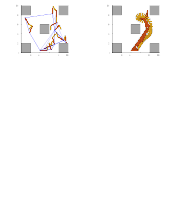
\includegraphics[width=1\linewidth]{figures/EXP2-2.pdf}
     \end{center}
     \vspace{-1em}
     \caption{Two-link robot having a resultant path that has a single node.}
     \label{two-link-2}
     \vspace{-1em}
\end{figure*}


\begin{figure*}[b]
    \vspace{-1em}
    \begin{center}
        \includegraphics[width=1\linewidth]{figures/NO-SOLUTION.pdf}
     \end{center}
     \vspace{-1em}
     \caption{Two-link robot on a grid obstacle, the solution cannot be found.}
     \label{no-solution}
     \vspace{-1em}
\end{figure*}

\subsection{\fontsize{10}{13}\selectfont EXPERIMENT-3}
In the following experiment, a more challenging map is introduced, featuring 16 obstacles arranged in a grid pattern. The robot configuration consists of a two-link structure set. The sample count is systematically increased, reaching 500 samples with 50 neighbors in the final iteration.
However, the resulting roadmap, as depicted in Fig.~\ref{no-solution}, indicates the toughness of the challenge. Although the sample count appears to be quite adequate, the connections between the samples do not form a usable path. The resultant graph is disjoint, compromising isolated islands that are not effectively connected. This observation underscores the delicate balance in selecting appropriate parameters, as a high sample count alone does not guarantee a well-connected roadmap. The interplay between sample count, neighbor number, and environmental constraints plays a crucial role in the algorithm's ability to navigate and connect configurations effectively. Adjustments may be necessary to achieve a more connected and usable roadmap in such challenging scenarios.

\begin{figure*}[bh!]
    \begin{center}
        \includegraphics[width=0.8\linewidth]{figures/TARS-2.pdf}
     \end{center}
     \vspace{-1em}
     \caption{The roadmap for TARS case, notice the graph lies on the ground where the base are sampled}
     \label{tars-2}
     \vspace{-1em}
\end{figure*}

\begin{figure*}[bh!]
    \begin{center}
        \includegraphics[width=0.8\linewidth]{figures/TARS-1.pdf}
     \end{center}
     \vspace{-1em}
     \caption{The resultant path that adheres to the constraints set through sampling.}
     \label{tars-1}
     \vspace{-1em}
\end{figure*}

\section{\large \textbf{Observations}}
The preceding series of experiments revealed several key insights. Firstly, it demonstrated that optimality can be achieved through the probabilistic roadmap (PRM) algorithm, sometimes with relative ease. Interestingly, environmental factors, such as increased constraints in the space, can have varied effects, and in the case of the PRM algorithm, certain constraints can actually be advantageous, simplifying the problem-solving process. Furthermore, it was observed that a higher number of samples and closer neighbors tend to result in a more optimal path. However, an increase in node changes along the path, especially near the goal, may lead to unwanted transients. In such cases, a less optimal path where the robot can stretch its "arms" might be preferred.

Additionally, certain problems become notably challenging when the configuration of obstacles is altered. Cases with more spread obstacles tend to be harder to solve, emphasizing the increased complexity introduced by changing the arrangement of obstacles. Nevertheless, the total obstacle-free space can be significantly larger in such instances compared to previous examples.

\section{\large \textbf{TARS Scenario}}

In the final experiment, the environment is constrained to the vertical plane. The robot configuration is designed to resemble two-links and three-feet robot, drawing inspiration from the TARS robot in the movie Interstellar (as depicted in Fig.~\ref{tars-fig}). The planning task is further constrained by requiring the TARS projection onto the vertical 2D plane to navigate along a specified course with various obstacles situated at different elevations.

The specific constraints imposed on the TARS robot in the vertical plane introduce a more realistic representation of its movement, aiming to incorporate gravity effects. The key constraint is that TARS should have at least one or two feet on the ground during its traversal from the initial to the goal configuration. This constraint mimics the influence of gravity, preventing the robot from freely moving in the air.

\begin{figure}[t]
    \begin{center}
        \includegraphics[width=0.68\linewidth]{figures/TARS-FIG.pdf}
     \end{center}
     \vspace{-1em}
     \caption{TARS robot from Imterstellar, which has the rectangular structure with rigid joints.}
     \label{tars-fig}
     \vspace{-1em}
\end{figure}

To enforce this constraint, a sampling strategy is integrated into the local planner section of the algorithm. The robot is consistently sampled from a set of points that lie on the ground. These points are derived from the ground obstacle, with a slight offset to mitigate potential collisions. This sampling strategy ensures that the robot maintains contact with the ground throughout its motion.

Additionally, a noteworthy aspect of the sampling process is the variation in the sampled leg that touches the ground. This variation enables the robot to alter its ground foot throughout the path, enhancing its adaptability to different configurations and scenarios. By incorporating these constraints and sampling strategies, the algorithm ensures that TARS moves in a physically plausible manner on the vertical plane, adhering to the specified constraints while navigating through the environment.


\section{\large \textbf{Conclusions}}
The exploration of stochastic methods in robot motion control, particularly focusing on the probabilistic roadmap (PRM) algorithm, has demonstrated its effectiveness in navigating complex configuration spaces. Random sampling within the free configuration space, coupled with local planning and collision checks, forms the basis of PRM. This paper focuses on the implementation details of a PRM planner designed for a planar two-link robot navigating within a polygonal world. The experiments conducted aim to provide a comprehensive understanding of the method's performance and adaptability in constrained environments.

The PRM approach proves to be versatile and scalable, accommodating diverse robot configurations and environmental conditions. The foundational steps involve precise problem definition, considering robot configurations and workspace configurations. The configuration space, represented as R2 * S1 * S1* ... * S1, enables flexibility in altering individual link lengths and widths, allowing for a variety of robot topologies.

The experiments, ranging from a single bar navigating a plane to a more complex two-link robot on a grid obstacle, offer valuable insights. Optimality is attainable through the PRM algorithm, with the adaptability to varying environmental constraints. The impact of sample count and neighbor number is evident, with higher values generally leading to more optimal paths but potentially introducing undesired transients.

The challenges posed by altered obstacle configurations highlight the algorithm's sensitivity to environmental changes. Spread obstacles increase the complexity, emphasizing the trade-off between obstacle distribution and total obstacle-free space. The experiment involving a TARS-like robot in a vertical plane further underscores the adaptability of the PRM approach to unique scenarios, navigating along specified courses with obstacles at different elevations.

In conclusion, the probabilistic roadmap algorithm stands as a successful motion planner, suitable for navigating unrestricted worlds and intricate robot configurations. The experiments showcase its capabilities, paving the way for further exploration and refinement in future work.

\bibliographystyle{bib/IEEEtaes}

\bibliography{bib/refs}\ %IEEEabrv instead of IEEEfull

\end{document}
